\PassOptionsToPackage{xetex}{xcolor}
\PassOptionsToPackage{xetex}{graphicx}
\documentclass[a4paper,landscape,headrule,footrule,xetex]{foils}

%%
%%%  Macros
%%%
\newcommand{\logo}{~}
\MyLogo{HG8011 (2019)}
\newcommand{\Story}{\SHA{HOUN}{The Hound of the Baskervilles}}

\newcommand{\header}[3]{%
\title{\vspace*{-2ex} \large Detecting Meaning with Sherlock Holmes\thanks{Creative Commons Attribution License: you are free to share and adapt as long as you give appropriate credit and add no additional restrictions: 
\protect\url{https://creativecommons.org/licenses/by/4.0/}.}
%\footnotemark
\\[2ex] \Large  \emp{#2} \\ \emp{#3}}
\author{\blu{Francis Bond}   \\ 
\normalsize  \textbf{Division of Linguistics and Multilingual Studies}\\
\normalsize  \url{http://www3.ntu.edu.sg/home/fcbond/}\\
\normalsize  \texttt{bond@ieee.org}}
 \date{Location: LT25}
 \renewcommand{\logo}{#2}
 \hypersetup{
   pdfinfo={
     Author={Francis Bond},
     Title={#2},
     Subject={HG8011: Detecting Meaning with Sherlock Holmes},
     Keywords={Semantics, Pragmatics, Meaning},
     License={CC BY 4.0}
   }
 %  pdfcopyright={Copyright © Francis Bond. Creative Commons 4.0 Attribution License.}
 %  pdflicenseurl={http://creativecommons.org/licenses/by/4.0/}
 }
}
%%
%% Multilingual Stuff
%%
\usepackage[a4paper,landscape,margin=25mm]{geometry}

\usepackage{fontenc}
\usepackage{polyglossia}
\setmainlanguage{english}
\setmainfont{TeX Gyre Pagella}
\usepackage{xeCJK}
\setCJKmainfont{Noto Sans CJK SC}
\setCJKsansfont{Noto Sans CJK SC}
\setCJKmonofont{Noto Sans CJK SC}
%\setCJKttfont{Noto Sans CJK SC}
%\setCJKmainfont{WenQuanYi Micro Hei}
%\clearpage
%\setCJKmainfont{AR PL SungtiL GB}

\usepackage[xetex]{xcolor}
\usepackage[xetex]{graphicx}
\newcommand{\blu}[1]{\textcolor{blue}{#1}}
\newcommand{\grn}[1]{\textcolor{green}{#1}}
\newcommand{\hide}[1]{\textcolor{white}{#1}}
\newcommand{\emp}[1]{\textcolor{red}{#1}}
\newcommand{\txx}[1]{\textbf{\textcolor{blue}{#1}}}
\newcommand{\lex}[1]{\textbf{\mtcitestyle{#1}}}

\usepackage{pifont}
\renewcommand{\labelitemi}{\textcolor{violet}{\ding{227}}}
\renewcommand{\labelitemii}{\textcolor{purple}{\ding{226}}}

\newcommand{\subhead}[1]{\noindent\textbf{#1}\\[5mm]}

\newcommand{\Bad}{\emp{\raisebox{0.15ex}{\ensuremath{\mathbf{\otimes}}}}}
\newcommand{\bad}{*}

\newcommand{\com}[1]{\hfill \textnormal{(\emp{#1})}}%
\newcommand{\cxm}[1]{\hfill \textnormal{(\txx{#1})}}%
\newcommand{\cmm}[1]{\hfill \textnormal{(#1)}}%
\usepackage{amssymb}
\usepackage{relsize,xspace}
\newcommand{\into}{\ensuremath{\rightarrow}\xspace}
\newcommand{\ent}{\ensuremath{\Rightarrow}\xspace}
\newcommand{\nent}{\ensuremath{\not\Rightarrow}\xspace}
\newcommand{\tot}{\ensuremath{\leftrightarrow}\xspace}
\usepackage{url}
\usepackage[hidelinks]{hyperref}
\hypersetup{
     colorlinks,
     linkcolor={blue!50!black},
     citecolor={red!50!black},
     urlcolor={blue!80!black}
}
%\usepackage{hyperxmp}
\newcommand{\lurl}[1]{\MyLogo{\url{#1}}}

\usepackage{mygb4e}
\let\eachwordone=\itshape
\newcommand{\lx}[1]{\textbf{\textit{#1}}}
\newcommand{\ix}{\ex\it}

\newcommand{\cen}[2]{\multicolumn{#1}{c}{#2}}
%\usepackage{times}
%\usepackage{nttfoilhead}
\newcommand{\myslide}[1]{%
\foilhead[-25mm]{\raisebox{12mm}[0mm]{\emp{#1}}}%
\leftheader{}%
\MyLogo{\logo}}

\newcommand{\mytask}[1]{%
\foilhead[-25mm]{\raisebox{12mm}[0mm]{\emp{#1}}}
\leftheader{🔍 Hi}%
\MyLogo{\logo}}

\newcommand{\myslider}[1]{\rotatefoilhead[-25mm]{\raisebox{12mm}[0mm]{\emp{#1}}}}
%\newcommand{\myslider}[1]{\rotatefoilhead{\raisebox{-8mm}{\emp{#1}}}}

\newcommand{\section}[1]{\myslide{}{\begin{center}\Huge \emp{#1}\end{center}}}

\usepackage{tcolorbox}
% \newcommand{\task}{\marginpar{\raisebox{-1ex}{\large
%       \tcbox[colframe=red,colback=white,arc=3pt]{\textbf{?}}}}}
% \newcommand{\task}{\marginpar{\raisebox{-1ex}{
%       \hspace{-0.5em}\tcbox[colframe=red,colback=white,arc=3pt]{%
%         
\includegraphics[width=1.5em]{pics/detective}}}}}
\newcommand{\task}{\marginpar{\raisebox{-2ex}{
      \hspace{-0.5em}\reflectbox{
\includegraphics[width=2em]{pics/detective}}}}}

\usepackage[lyons,j,e,k]{mtg2e}
\renewcommand{\mtcitestyle}[1]{\textcolor{teal}{\textsl{#1}}}
%\renewcommand{\mtcitestyle}[1]{\textsl{#1}}
\newcommand{\chn}{\mtciteform}
\newcommand{\cmn}{\mtciteform}
\newcommand{\iz}[1]{\textup{\texttt{\textcolor{blue}{\textbf{#1}}}}}
\newcommand{\con}[1]{\textsc{#1}}
\newcommand{\gm}{\textsc}
\newcommand{\cmp}[1]{{[\textsc{#1}]}}
\newcommand{\sr}[1]{\ensuremath{\langle}#1\ensuremath{\rangle}}
\usepackage[normalem]{ulem}
\newcommand{\ul}{\uline}
\newcommand{\ull}{\uuline}
\newcommand{\wl}{\uwave}
\newcommand{\vs}{\ensuremath{\Leftrightarrow}~}
%%%
%%% Bibliography
%%%
\usepackage{natbib}
%\usepackage{url}
\usepackage{bibentry}


%%% From Tim
\newcommand{\WMngram}[1][]{$n$-gram#1\xspace}
\newcommand{\infers}{$\rightarrow$\xspace}



\usepackage{rtrees,qtree}
\renewcommand{\lf}[1]{\br{#1}{}}
\usepackage{avm}
%\avmoptions{topleft,center}
\newcommand{\ft}[1]{\textsc{#1}}
%\newcommand{\val}[1]{\textit{#1}}
\newcommand{\typ}[1]{\textit{#1}}
\avmfont{\sc}
%\avmvalfont{\sc}
\renewcommand{\avmtreefont}{\sc}
\avmsortfont{\it}


%%% From CSLI book
\newcommand{\mc}{\multicolumn}
\newcommand{\HD}{\textbf{H}\xspace}
\newcommand{\el}{\< \>}
\makeatother
\long\def\smalltree#1{\leavevmode{\def\\{\cr\noalign{\vskip12pt}}%
\def\mc##1##2{\multispan{##1}{\hfil##2\hfil}}%
\tabskip=1em%
\hbox{\vtop{\halign{&\hfil##\hfil\cr
#1\crcr}}}}}
\makeatletter

\newcommand{\sh}[1]{\lowercase{\href{https://fcbond.github.io/sh-canon/#1.html}}{#1}}
\newcommand{\SHA}[2]{\lowercase{\href{https://fcbond.github.io/sh-canon/#1.html}}{\textit{#2}}}

\newcommand{\tra}[1]{\textcolor{olive}{\textsf{#1}}}
\usepackage{multicol}
\usepackage{booktabs,subscript}
\newcommand{\DF}[1]{\parbox{.6\textwidth}{#1}}
\begin{document}
\makexeCJKinactive
\renewcommand{\avmvalfont}{\it}
\header{~}{Reading Sherlock Holmes I}{\normalsize based on slides by Jane Wong Y. C. }
\maketitle

%\include{schedule}


\myslide{Genre \& Historical Context}
\begin{itemize}

\item \txx{Genre}: The French term for a type, species, or class of
  composition. A literary genre is a recognizable and established
  category of written work employing such common conventions as will
  prevent readers or audiences from mistaking it for another kind.
  \item Modern detective fiction as genre:
    \begin{itemize}
    \item Biblical stories of  crime and punishment    
  \item Greek tragedy    
  \item Renaissance revenge tragedy (16th-17th   century)    
  \item Gothic horror stories   (early 19th century)    
  \item Victorian crime stories (early 19th to late 19th   century)
  \end{itemize}
\end{itemize}


\myslide{Genre \& Historical Context}
\begin{itemize}
  \item A story in which the principal action and focus of interest is
    the investigation of a crime \ldots  by a detective figure, either professional or amateur. The centrality of this detective figure distinguishes the detective story proper from some other kinds of crime fiction in which the emphasis lies upon the actions of a crime's perpetrator or victim.      
  \item Conventionally, the crime should be an especially baffling case that requires the uncommon ingenuity of the detective to find a solution and identify or pin the blame on the true perpetrator, who commonly has an apparently safe alibi or has left a false trail incriminating others. Various kinds of crime are possible subjects, although murder, and preferably multiple murder involving the elimination of witnesses to the original crime, has been found to be the most appetizing to readers addicted to the genre.       
  \item All references to genre from   \textit{The Oxford Dictionary of
    Literary Terms} (ODLT), 3rd   Edition (Chris
   Baldick)

  \end{itemize}


  \myslide{Genre \& Historical Context}
\begin{itemize}

  \item  Dorothy Sayers  identifies 4 early stories with the elements of the
    detective story (CF) 
    \begin{itemize}
    \item    Two from the Old Testament from the Book of
    Daniel
  \item     One from Herodutus   
  \item   Another from the Hercules myths
    (classical mythology)    
  \end{itemize}

\item According to Sayers, common elements of these early stories
  include: 
  \begin{enumerate}
  \item A crime that has been committed
  \item “Locked-room mystery” involving an apparently impossible crime
    perpetrated within an enclosed space with ostensibly no exit or
    entrance (Poe's   Rue Morgue   story being an example)
  \item Tampering of evidence
  \item False accusations
  \item Puzzles
  \item Uncovering truth 
  \end{enumerate}
\end{itemize}

  \myslide{Genre \& Historical Context}
\begin{itemize}
  \item Some critics object to Sayer’s categorization of early elements of the detective story. 
  \item Julian Symons argues that while stories from the bible and
    Herodutus include puzzles, and that even though “puzzles are an
    essential element of the detective story, they are not detective
    stories in themselves” (CF 8)
  \item Symons main argument: the puzzles in the stories focus more on
    punishment than on detection:  
    \begin{quote}
      The emphasis on right conduct, reinforced by the harsh
      punishments meted out in the stories from the Book of Daniel, is
      characteristic of most narratives of crime up until the
      mid-nineteenth century, including the stories of Edgar Allan
      Poe \hfill (CF 8)
  \end{quote} 
\end{itemize}           
\myslide{Elizabethan Revenge Tragedies (16th-17th c.)}
\begin{itemize}
\item   Preoccupied with the restoration of social order, “as
  embodied by the act of revenge.” 
\item    “The revenge pattern of injury and retribution creates a
  narrative in which the unity of justice and order prevails.” 
\item    It is ironic that revenge narratives are produced when there is a lack
  of justice. 
\item    “The revenger pursues a course of action that is
  itself unjust, in an attempt to restore the unity and social order
  that justice promises” but have failed.
\item     Francis Bacon refers to
  the early developments of the revenge tragedy as “a kind of wild
  justice” (CF 11)

\end{itemize}
\newpage
\begin{itemize}
\item According to Gamini Salgado, there is a 5-part structure to
  Elizabethan revenge tragedies, and they are parallel to early Greek
  Senecan tragedies.
\item  This structure is also commonly used in modern
  crime fiction today: 
  \begin{enumerate}
\item   Exposition     
\item  Anticipation      
\item  Confrontation 
\item  Partial execution 
\item  Vengeance (CF  11)
\end{enumerate}      
\end{itemize}

\myslide{The Newgate Calendar}
\begin{itemize}
\item In the 18th century, the \href{http://www.exclassics.com/newgate/ngintro.htm}{Newgate Calendar} stories provided the
  first large collection of cautionary tales; accounts of criminals
  arrested, tried, and punished captured popular imagination.   
\item Originally a monthly bulletin of executions, produced by the
  Keeper of Newgate Prison in London
\item Then expanded with bibliographies and descriptions of crimes
\item Rise in crime during the Industrial Revolution; large population shift from rural to urban areas; also caused by high unemployment rates.       
  \item “Thief-takers” as predecessors to police; the Metropolitan Police Act in 1828 established a police force.        
  \item Invention of photography in 1839; development of forensic sciences. 
  \end{itemize}
\newpage

\begin{center}
  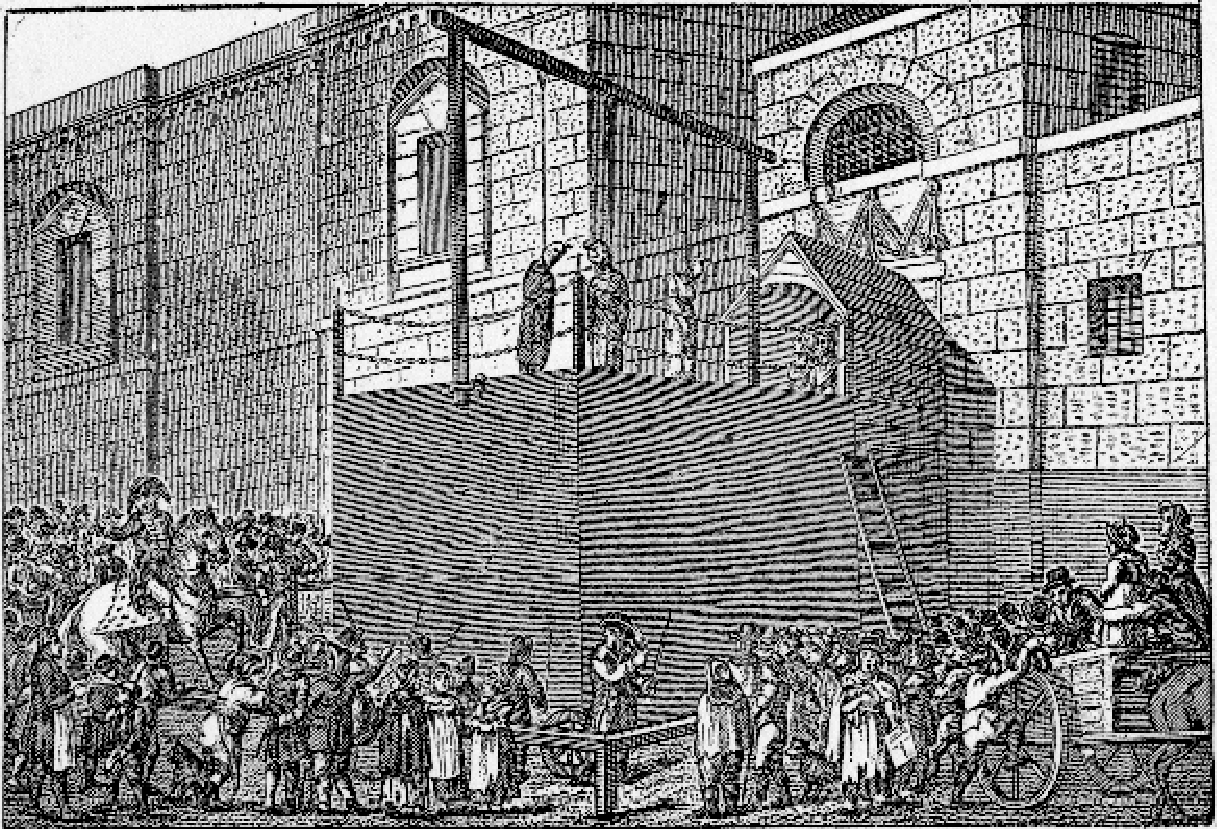
\includegraphics[width=0.8\textwidth]{pics/newgate4}

  An Execution at the Debtor's Door of Newgate
\end{center}

\myslide{The Golden Age of Detective Fiction}
\begin{itemize}

  \item The Golden Age in Britain started in 1920, with Agatha
    Christie’s first novel \textit{The Mysterious Affair at Styles}
    and finished with WWII.
    \item  Country-house murder synonymous with the whodunnit.
    \item    Classic British whodunnit: “character is usually
      sacrificed in favour of ingenious plotting, as the puzzle
      element of the challenge to the reader to discover ‘whodunnit’
      before the book reveals it, is emphasized.”  
    \item Four main authors
      \begin{itemize}
      \item Agatha Christie: Hercule Poirot and Miss Marple
      \item Dorothy L. Sayers: Peter Whimsey (younger brother of a duke)
      \item Margery Allingham: Albert Campion (viscount)
      \item Ngaio Marsh: Roderick Alleyn (brother of a baronet, and policeman)
      \end{itemize}
    \end{itemize}
    \newpage
\myslide{Across the Pond}
\begin{itemize}
 \item Hard-boiled detective stories — USA
      \begin{itemize}
      \item  Does not use appeal and reason or logic and focuses on the
        detective character “normally characterised by violence and
        betrayal.”
        \begin{itemize}
        \item Dashiell Hammett (1894–1961): Sam Spade, the Continental Op
        \item Raymond Chandler (1888–1959): Phillip Marlowe
        \item Mickey Spillane (1918–2006): Mike Hammer
        \end{itemize}
      \end{itemize}
    \item Sherlock Holmes also very popular!
    \end{itemize}

  
\myslide{Post Golden Age}
\begin{itemize}
  \item  By the 1970s [post war generation], the aristocratic
      elements diminished in British detective stories and they
      developed more along the lines of hard-boiled American
      narratives; detectives are associated with professional police
      enforcement agencies.  
    \item Police Procedurals --- more emphasis on the process
      \begin{itemize}
      \item Ed McBain: 87th Precint
      \end{itemize}
    \item Crime Thrillers --- more emphasis on the criminal
      \begin{itemize}
      \item Thomas Harris: Hannibal Lector \textit{The Silence of the Lambs}
      \end{itemize}
    \item Historical Crime Fiction --- set in the past; a blend of
      genres
      \begin{itemize}
      \item Umberto Eco: William of Baskerville \textit{The Name of
          the Rose}
      \end{itemize}
 \end{itemize}

\section{The Adventure of the Speckled Band   (1892)}
\myslide{The Adventure of the Speckled Band}




The Story (like most) is narrated by Watson
\begin{enumerate}
  \item  act[s] as a contrast to the abilities of the detective, emphasising in the detective's genius a difference in degree, rather than a difference in kind
  \item  act[s] as recorder, not only of the story, but also the physical data upon which the detective’s analytic ability depends
  \item  embod[ies] the social and ideological norms of the period
  \item  masks information from the reader because Watson is limited in knowing what Holmes discovers when he is away, or of knowing what Holmes is thinking.
  \end{enumerate}
  \begin{itemize}
  \item The narrator feeds the clues to the reader
  \item But are they credibile?
  \end{itemize}

\myslide{Story as a window on society}
\begin{itemize}           
  \item Representation of social class, culture, and gender.     
  \item Holmes as distinctly English (East India 1757-1858; Crown rule 1858-1947).      
  \item Holmes and Roylott of Stoke Moran (Surrey); English aristocracy as a backdrop here, highlighted by the family’s historical past, and how the family’s wealth went through different phases.     
  \item Watson’s emphasis that Holmes is not interested in money, and
    Holmes’ reassertion to the same: “As to my reward, my profession
    is its reward.” 
  \end{itemize}

\myslide{Hero vs Villain}
\begin{itemize} 

  \item Watson’s depiction of Holmes
    \begin{quote}
      “I had no keener pleasure than in following Holmes in his
      professional investigations, and in admiring the rapid
      deductions, as swift as intuitions, and yet always founded on a
      logical basis, with which he unravelled the problems which were
      submitted to him.”
    \end{quote}
  \item Holmes as the “perfect” English man; British empire
  \item Dr. Roylott’s history and his qualities
  \item Reading Dr. Roylott alongside the colonial narrative;
    assumptions of those who spend time in India and are too friendly
    with the natives
   
\item Dr. Roylott’s behavior and his temperament
\\ even his name gives it away: Dr. \ul{Grimesby} Roylott
  \end{itemize}

\myslide{Britain vs the Other}
\begin{itemize}
\item Dr. Roylott’s past in India is an important thread throughout
  the story. 
\item The exotic realm of India is associated with wickedness. 
\item The region is
  considered partially responsible for his violent temperament.
 As Helen remarks, Dr. Roylott’s “violence of temper approaching to
 mania has been \ldots{} intensified by his long residence in the tropics.”
\item  The 
  creatures imported from India are dangerous:

  \begin{quote}
The idea of a snake instantly occurred to me, and when I coupled it
with my knowledge that the doctor was furnished with a supply of
creatures from India, I felt that I was probably on the right
track. The idea of using a form of poison which could not possibly be
discovered by any chemical test was just such a one as would occur to
a clever and ruthless man who had had an Eastern training \ldots{}  
\end{quote}

\end{itemize}
\myslide{Men vs Women}
\begin{itemize}
  \item If the two male characters (Holmes and Roylott) stand on opposite end of the spectrum then we do we make of the women in the stories?      
  \item Tensions; male and female spaces: “Was it your custom to always lock yourselves in at night?”        
  \item The “locked-door” mystery.        
  \item Helen Stoner approaches Holmes for help; her sister’s death
    and her appeal to Holmes contributes to the construction of Holmes
    as a hero figure, and specifically, Holmes' masculinity as
    something that overcomes cowardice. 
    (Consider the scene of Roylott’s confrontation of Holmes.)      
  \item Helen’s trust in Holmes and his access of the female space
  \item Necessity; Holmes has access to the room and the description of Julia’s bed being clamped down to the floor is troubling.
  \end{itemize}

\myslide{The conclusion}
\begin{itemize}
\item Possibly the most popular of the stories
\item A classic locked room mystery
  \begin{itemize}
  \item typical \txx{red herring} ``misleading clue'': the \ul{band} of gypsies
  \end{itemize}  \item In solving the puzzle, Holmes in effect restores order
    \begin{itemize}
    \item the order that has disrupted gender assumptions, civility (in removing
    the threat of that which is uncontrollable, corrupt, violent,
    etc.)
  \item the damsel is freed from her distress and the villain gets his just deserts. 
  \end{itemize}
\item The punishment comes naturally, not through the legal
  system

\end{itemize}
\myslide{Bibliography}
  \begin{itemize}
  \item   John Scaggs (2005) \textit{Crime Fiction} (CF), Routledge
  \end{itemize}

\end{document}

%%% Local Variables: 
%%% coding: utf-8
%%% mode: latex
%%% TeX-PDF-mode: t
%%% TeX-engine: xetex
%%% End: 

